\chapter{Use Case: Supply Chain Management}
\section{Supply chain management}
Supply chain is a amount of activities that information flow product form suppliers to customers, manage all activities related to sourcing, conversions, delivery and etc. Supply chain management, not only is beneficial in various Fields such as financial, social and world. It enhances resources, exploitation and cyclic time from material to end users.
Supply chain processes started within the company’s processes or distribution. We believe that supply chain management is essential for the delivery of business results\cite{Wu}.
\begin{center}
	\begin{figure}[htb!]
		\begin{minipage}{0.50\linewidth}
			
			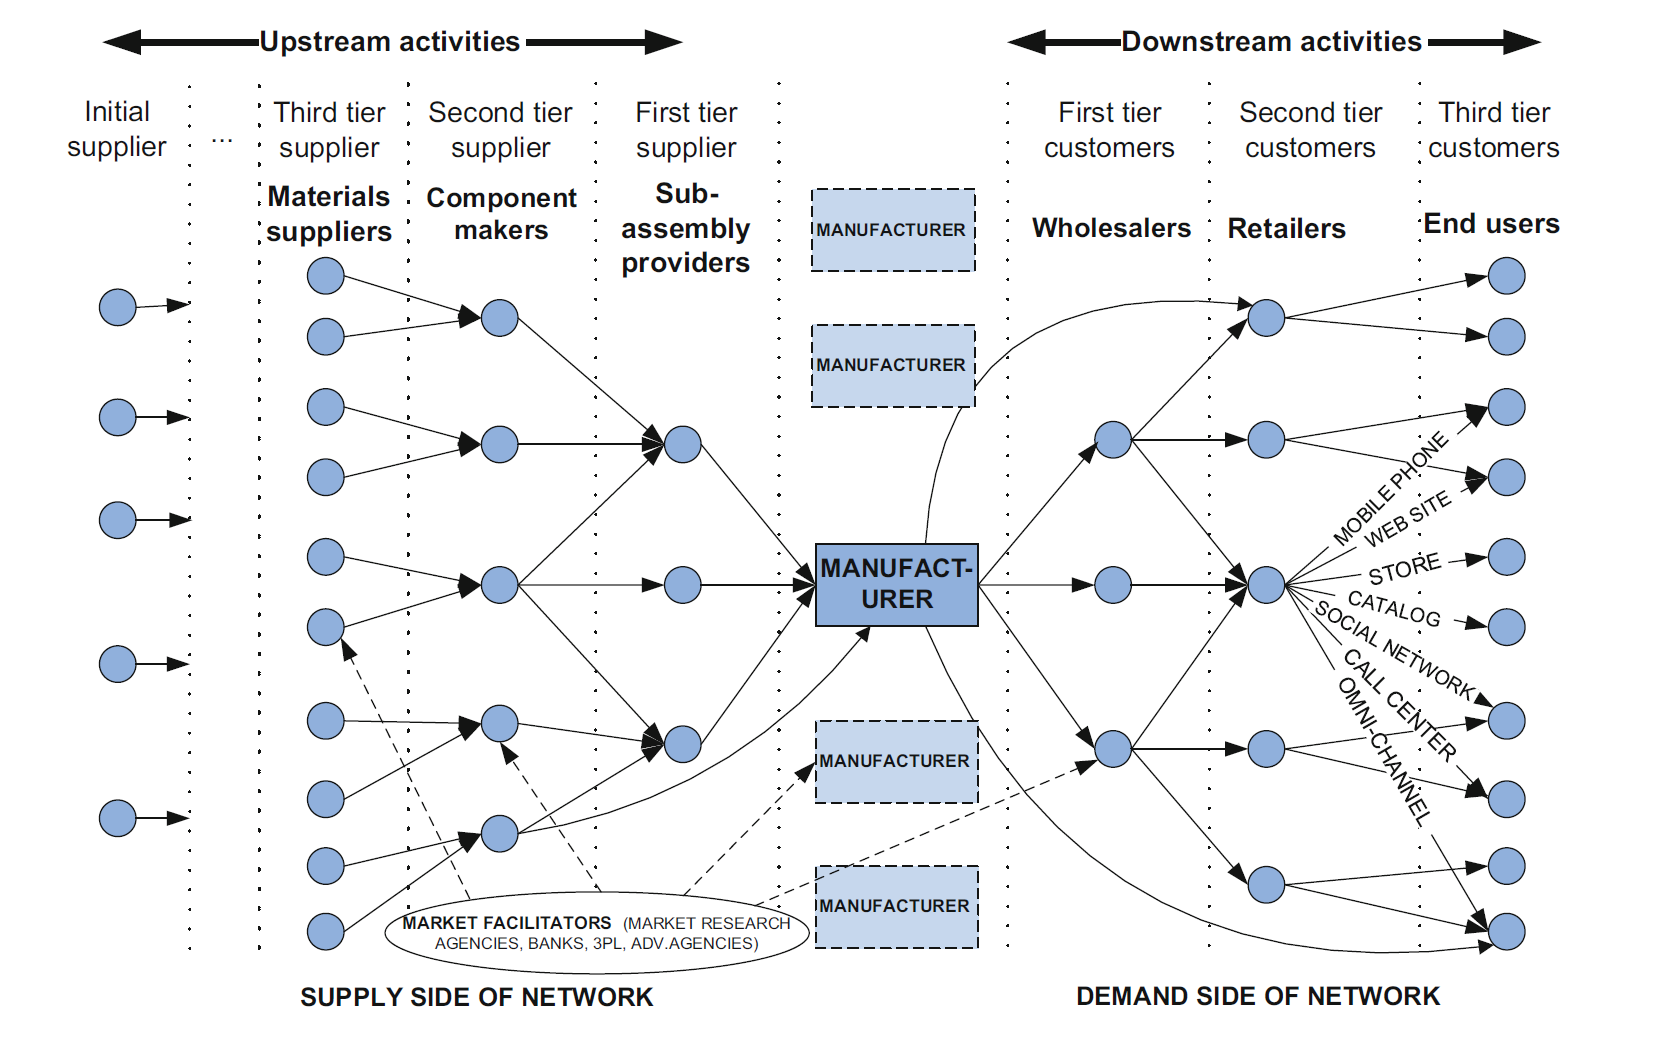
\includegraphics[width=1.85\textwidth]{images/chap03_SCM_network.png}
		\end{minipage}
		\caption{Network supply chain management\cite{Sajter}}	
	\end{figure}	
\end{center}

Supply chain management is critical factor in global business and improvement effort become increasingly important. Supply chain management is an great strategy that make alignment flow of raw material, manufacturing, and distribution to customer according to customers demand. \\
Supply chain management is an approach that integrate the network of operating entities to delivery system fulfilling the satisfaction of customer and protecting the competitiveness of supply chain. 
In this regards, Supply chain is the chain of activities and demand marketing service\cite{Kemal}. Christopher (TODO) claimed against uni-dimensional supply chain as follow:\\
\textit{"Supply chain management should be termed demand chain management to reflect the fact that the
chain should be driven by the market, not by suppliers. Equally the 'chain' should be replaced by
'network' since there will normally be multiple suppliers and, indeed, suppliers to suppliers as well as
multiple customers and customers to be included in the total system."}
\section{How to improve SCM applying blockchain? }
The decentralized nature of blockchain couple with data immunity made it appropriate for supply chain management.
This feature provides opportunity to fulfill requirements of supply chain.  
Using blockchain, from one hand store data on supply chain, thus data can not tampered easily. On the other hand, data from multiple stack holders can be integrated into blockchain rather then stored in individual system.
One of the critical factor in supply chain management, manufacturing management, delivery management, is data management. The type of data in supply chain is not bounded to inventory information. Data steaming is as core process in supply chain management.
\begin{center}
	
	\begin{figure}[htb!]
		
		\begin{minipage}{0.55\linewidth}
			
			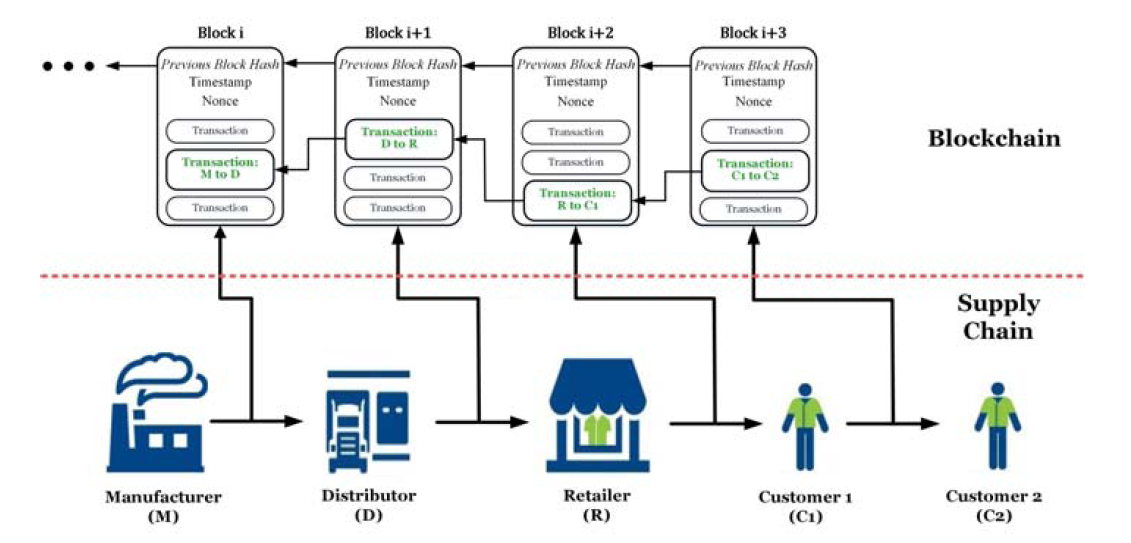
\includegraphics[width=1.85\textwidth]{images/chap03_SupplyChain_blockchain.png}
		\end{minipage}
		\caption{Supply chdain management with blockchain\cite{Nazmul}}
		
	\end{figure}
	
\end{center}
Data for SCM fed into blockchain via information flow. In this process information flow previous input and stack holders store data in off-line way. Information can exchange through postal system. One possible way is to automate information flow, but it brings some concerns such as manipulation of data veracity and violate security and time consuming of data processing. Therefore, we can improve SCM system by sharing, information within supply chain, protect data veracity and accelerate the data recovery.\\
 But there are some issues to do this, one of them is to gather data from external environment convert to digital information via IoT devices, smart sensors and etc. The other is to identify how implement blockchain on SCM through various approaches. So that, they can obtain more requirement of SCM from industry.\\
Generally, critical property of blockchain which is decentralization cause to deal with three concerns such as Trust-less, security, and authentication. We deal with these issues in SCM by traceability, efficiency and transparency.
Blockchain application is on increase in payment infrastructure, cryptocurrency and verification. In supply chain management, blockchain not only offers transparency regarding who is participating and which action take place, but also provide solutions for real-time supplier management, shipment management, identity management and etc. Blockchain is beneficial to all parties and supply chain network. \\

\subsection{Blockchain operation in supply chain management}
The main benefits of blockchain technology application have been concerned on how it can
provide valid information to supply chain network participants.  The need for collective activities will disapear, Through such transparent  information sharing mechanisms.
Participants can rely on transaction history to transfer assets like ether, even without needing to third party\cite{Nina}.
Blockchain emphasized on four attributes:
1. Information synchronization: all participants has access to same data containing history of transaction.\\
2. p2p network and consensus mechanism: there is no need to third authority to control transactions\\
3. Smart contact: all obligations are formalized in programming code which should be met.\\
4. Data stability: Modification must be verified just with consensus of all participants, Not altering without collective verification\cite{Nina}. \\
Based on Four common attributes of blockchain
 summarized in table follow:\\
 \begin{table}[h!]
 \begin{center}
   \begin{adjustwidth}{-1cm}{}
	
 	\begin{tabular} { c | c | c | c | c | c }
 			
 		\tiny \textbf{Context} &\tiny \textbf{Logistic}\cite{Tijan} & \tiny \textbf{HealthCare} & \tiny \textbf{Banking}\cite{Guo} & \tiny \textbf{Engineering}\cite{Kontantinos} & \tiny \textbf{Green SCM}\cite{Sarkis} \\
 		\hline
 		\tiny \makecell{Information\\ synchronization} & \tiny \makecell{digital version\\ of a ledger to\\ decentralized\\ system participants\\ to follow data} & \tiny \makecell {Allow copies of\\ patient's record\\ to update with \\participants records} & \tiny \makecell{Remove link of \\third party financial\\ institution\\ in distribution\\ of goods} & \tiny \makecell{participants interact\\ with blockchain via\\ private and\\ public key} & \tiny \makecell{all participants\\ have same copy\\ of ledger which\\ is updatable\\ by new modification \\in blockchain}\\ 
 		\hline 
 		\tiny P2P network   & \tiny \makecell{participants share \\transaction with\\ blockchain and\\ copy of ledger}& \tiny \makecell{Participants have \\copy of whole\\ blockchain to\\ ensure that \\date is authenticated} & \tiny \makecell{Helping system\\
 		participants control \\big data and
 		\\constructing ownership} & \tiny \makecell{transaction broadcast \\into blockchain via \\user's node} & \tiny \makecell{Participants can\\ follow record of\\ transaction, thus\\ can track performance \\of transportation}\\ 
 		\hline
 		\tiny Smart contract   & \tiny \makecell{legal provision\\ are formalized\\ into code and\\ verified through a \\network of peers } & \tiny \makecell{records stored on\\ blockchain } & \tiny \makecell{ensure that\\ payment is\\ done automatically\\ after reaching\\ result and\\ reduce manual\\ risk} & \tiny \makecell{script storing\\ in blockchain\\ is similar to stored\\ procedure in\\ relational database\\ management system} & \tiny \makecell{Automatic payment\\ is done, when\\ regulations are\\ met or value\\ added to products}\\ 
 		\hline
 		\tiny Data stability   & \tiny \makecell{ transaction are\\ approved by\\ consensus of all\\ participants, it \\stores in block } & \tiny \makecell{Create indecomposable \\databases for medical \\records and tracing\\
 		pharmaceuticals\\ through manufacturing\\
 		and distribution} & \tiny \makecell{after entering\\ information into\\ system, can not\\ be altered, thus preventing\\ from subsequent\\ fraud} & \tiny \makecell{transaction will\\ be verified\\ through hash\\ of previous block\\ in blockchain} & \tiny \makecell{Tracing the waste, \\distribution\\ responsibility to\\ system participants \\for cleanup\\ cost}
 	    
 	   
	 		
 	\end{tabular}
  \end{adjustwidth}
 \caption {Summary of blockchain characteristics in various contexts supply chain management.}
 \end{center}
\end{table}

\subsection{Analysis of supply chain ontology models}

This section reports on the analysis using the comparison
framework. The analysis presented here provides insights about
the gaps in existing supply chain ontology research. Table lists these ontologies shows the
values for the criteria application, scope, KR paradigm, language and methodology approach.\\
\textit{Scope} concerns with the field of industry which used in ontology.\\
\textit{Language} is the type of language that is used in ontology.\\
\textit{Application} is concerned with the type of problem-solving task for which the ontology is to be used.
These tasks span a wide range of applications in supply chain.\\
\textit{Key concept} is about main concept used in ontology.\\
\textit{Purpose} concern with the goal of using ontology using in supply chain\cite{Tonci}.\\ 


\begin{landscape}

\begin{table}[ht!]
	\begin{center}
		\begin{adjustwidth}{}{}
			\begin{tabular}{ c | c | c | c | c | c | c | c  } 
				
				\tiny \textbf{\makecell{Supply\\ chain\\ Ontology\\ model}} & \tiny \textbf{\makecell[l]{KR \\paradigm}} & \tiny \textbf{Language} & \tiny \textbf{Scope} & \tiny \textbf{Purpose} & \tiny \textbf{Key concept} & \tiny \textbf{\makecell[l]{Methodically\\ approach}} & \tiny \textbf{\makecell[l]{Application}}\\
				
				\hline  
				
				\tiny \textit{\makecell{Model by\\ Sousa at al.\cite{Sousa}}} & \tiny \makecell[l]{Algebra \\of sets} & \tiny UML & \tiny \makecell{Business\\ network} & \tiny \makecell[l]{Improve manufacturing \\performance of virtual \\enterprise by bridging \\gap between planing \\level and control level\\, integrating incoherent \\manufacturing systems}& \tiny \makecell[l]{plan, unit, product,\\ organization,\\ order, resource,\\ customer, activity.}&  \tiny \makecell[l]{Combination of generic\\ techno-organizational\\ requirement and synthesis\\ of ontology} & \tiny \makecell[l]{ Production and\\ operation planning \\virtual enterprise of\\ and control \\semiconductor industry}\\
				
				\hline
				
				\tiny \textit{\makecell{TOVE\\ ontology\cite{Kim}}} & \tiny DL  & \tiny \makecell{XML} & \tiny \makecell{internal \\ supply\\ chain} &\tiny \makecell[l]{Develop enterprise\\ model which will\\ have ability to deduce\\ answer queries in\\ industrial environment}  & \tiny \makecell[l]{agents, roles,\\ positions, activity,\\ resource, commitment,\\ communication,\\ authority} & \tiny \makecell[l]{Ontology developed\\ and comply to\\ pose competence\\ questions at \\the beginning} & \tiny \makecell[l]{Using TOVE \\model to analyze\\ enterprise\\ ontology}\\
				
				\hline
				
				\tiny \textit{\makecell{IDEON\\ ontology\cite{Madni}}} & \tiny \makecell[l]{Algebra \\of sets} & \tiny UML & \tiny \makecell[l]{inter-business \\network} & \tiny \makecell[l]{provides a common\\ foundation for designing,\\managing,
					and controlling\\ collaborative, distributed\\ enterprises} & \tiny \makecell[l]{process, organization, \\resource, enterprise, \\product} & \tiny \makecell[l]{there is no formal\\	evaluation, however\\ the ontology was\\ assessed based on\\ its actual uses\\ against the purposes.} & \tiny \makecell[l]{support multiple enter-\\prise
					applications: Crisis\\ Action Planning and\\ Integrated Product-Process\\ Development which enabled\\ systems engineering.} \\	 
				
				\hline
				
				\tiny \textit{\makecell{Model by \\Ye at al.\cite{Ye}}} & \tiny DL & \tiny \makecell[l]{OWL, SWRL} & \tiny \makecell[l]{inter-business\\ network} & \tiny \makecell[l]{serve as an interlingua\\ to enable
					information \\integration across interacting\\ applications and semantic\\ integration of heterogeneous \\system in supply chain} & \tiny \makecell[l]{structure, activity,\\ performance, purpose, \\role, party, transfer} & \tiny \makecell[l]{SCOR provides a basis\\ for
					describing the \\knowledge of supply chain\\ performance; The same\\ methodology for the\\ development of EO\\ was used} & \tiny \makecell[l]{application integration\\ framework based\\ on developed ontology\\ is used to solve\\ problem of information\\ integration}\\
				
				\hline
				
				\tiny \textit{\makecell{EAGLET\\ ontology\cite{Geerts}}} & \tiny \makecell[l]{} &\tiny UML & \tiny \makecell[l]{supply chain\\ of thing}& \tiny \makecell[l]{facilitate the visibility\\ and inter-operability of\\ things along the \\supply chain.} & \tiny \makecell[l]{Event,
					agent,\\ location, equipment,\\Thing}& \tiny \makecell[l]{Hybrid:inspiration, \\synthesis and \\ compliance of\\ this ontology with\\ real-world practices\\ is much higher.} & \tiny \makecell[l]{1. extend formalization\\ beyond current knowledge\\ 2. address more supply\\ chain practice; \\3. used as an instantiation\\ pattern; 4. focus\\ on fixed asset and\\ agent visibility} \\
				
				\hline
				
				\tiny \textit{\makecell{MSE ontology\cite{Lin}}} & \tiny DL & \tiny RDF, OWL & \tiny \makecell[l]{inter-business\\ network} & \tiny \makecell[l]{provide semantic and\\ syntactic interoprability\\ service to enable\\ understanding of basic\\ manufacturing terms \\between different \\manufacturing system\\ engineering enterprise \\applications} & \tiny \makecell[l]{product, enterprise,\\ project, process,\\ resource, strategy, flow} & \tiny \makecell[l]{built on the\\ experiences and\\ knowledge of \\published\\ manufacturing\\ system information\\ models.}    	
				& \tiny \makecell[l]{There are some \\application area\\ thereby companies\\ enter into tempoSEMrary\\ inter-enterprise\\ collaboration for\\ exchanging information} \\
				
				\hline
				
				\tiny \textit{\makecell{Enterprise \\ontology\cite{Uschold}}} & \tiny \makecell[l]{} & & \tiny \makecell[l]{not \\applicable}& \tiny \makecell[l]{facilitate enterprise\\ design and
					analysis by\\ supporting\\ communications among \\human} & \tiny \makecell[l]{person, activity,\\ plan, resource,\\ marketing,\\ organization, \\purpose, strategy} & \tiny \makecell[l]{inspiration and \\synthesis;\\
					ontology was assessed \\based on its uses\\ against the original\\ purposes.} & \tiny \makecell[l]{improve method with\\ a framework for \\integrating method and\\ tools which are\\ appropriate to enterprise\\ modeling and management \\of changes }
			\end{tabular}
			
		\end{adjustwidth}
	\end{center}
	\caption{Different supply chain ontology models}
\end{table}

	
\end{landscape}

\section{How smart contract improve supply chain}
Before era of smart manufacturing, supply chain management is and log process called as black box, in terms of input-output mechanism. This black box consist of multiple mini process related to product, services, customer and
etc. Many possible by emerging new technology like smart sensor and IoT devices, This long process are made more cost-effective, transparent. Meanwhile collaboration between supply chain structures bring strategic benefit to involve all parties.\\
Using some new technology in supply chain management such as smart contract, IOT devices and consensus mechanism in blockchain make this system more cost-efficient, efficient and secure at the same time. Smart contract can be implemented through out life-cycle of supply chain process of raw-material to end users. For instances, smart contract can be used in terms of demands of product personalization, utilization and services, subsequently automated payment machines that are connected to IOT can cooperate using smart contract in terms of requirement that must be met before going to next machine.\\
In additions, Based on blockchain with logic rules, smart contract can be used to control quality and cont management between company and Original Equipment Manufacture(OEM). Also manufacture can use smart contract with authorized provider in terms of how product should be repaired or updated and son on.\\ (blockchain based trust mechanisimm IOT)
Furthermore, Smart contract can simplicity the performance of supply chain and improve transparency across supply chain. Using IOT devices to track the locations  of goods. Smart contract can be helpful in this case determining the provenance of goods. This is important part in all industry special in food industries. recently, some big companies start using smart contract to trace the device racing the goods, including meet, foods, containers, and even diamond\cite{Adam}.

\section{How smart contract works?}

To understand how smart contract works?, the first we should know how Etheruem operates and how smart contract comes into play?
could any The main term of Etheruem is account, any time that there is exchange information between accounts, it captures in blockchain.\\
There are two accounts in Ethereum : One is externally owned account that controlled by private key, the other is contract account which is activated by EOA and controlled by internal code.\\
In order to create smart contract, participant should identify an opportunity to agree to other parties. This could any values such as good and service. Then they must set term and conditions that have to b met. This could be triggered by participants or external events. All agreement will be written in code as smart contract which can be deployed in blockchain where executed by first initiating contract.\\
To initiate smart contract, participant fulfill transaction with contract account which encrypted by private key and transmitted to other nodes in blockchain. The other participant verify transaction if it is triggered by valid participant. After all, the transaction is added to blockchain after obtaining consensus by majority.\\
Then, smart contract will be executed and recorded, finally, all nodes are updated in network. But already mentioned, the outcome not altered and just states of blockchain will change. Note that, every initiator has to pay for transaction fee to create changes in the state of Ethereum platform. The smart contract used in Ethereum to store information on blockchain securely\cite{Angwei}.\\

\section{Addressing supply chain using smart contract: }
Using blockchain guide to solve cooperation challenges in SCM. Blockchain improves the transparency and verification in supply chain and smart contract handle the exchanges between many participants and nodes in blockchain.\\
Smart contract can handle improve this issue three factors: Tractability, efficiency and transparency. \\
\begin{itemize}
	\item \textit{Transparency:} Supply chain improves traceability in supply chain by storing provenance of goods on blockchain. this will ensure the manufacture where goods, raw material are coming from valid sources and customer have more confident that purchase legal products.\\ 
	Another usage of smart contract in supply chain. In addition, transparent authentication across supply chain. Participant can verify easily each other using certification stored in blockcahin in digital form. All together, allow supply chain manager to have correct decision when selecting supplier to work with.\\
	\item \textit{Traceability:} Smart contract helps supply chain in terms of traceability in a way that it can easily trace the inventory at every long way From raw-material to end user delivery. The product can be traced using serial number, tags or smart sensors.\\
	With the growing of IOT, device can connected to each other. smart sensor provides some information such as location, environment, and quality of product. Another problem in supply chain process is that the goods will be depreciated when arriving to users due to delay. Smart contract attibutes ca mitigate delay , keeps the supply chain agile to be fully- equipped to cope with the product delivery distribution such as natural catastrophe and etc.\\
	As already mentioned, one of the main usage of smart contract is tracing the inventory in supply chain and facilitated the supply chain system to be track the products.\\
	 \item \textit{Efficiency:}  Smart contract can also improve the efficency of supply chain in a way that using self executed attibute of smart contract help supply chain to eliminate the paper work method and just executed smart contract onlyany time that obligations are met. Anther thins that using smart contract as code enhance the cost efficiency. because it eliminate numerous document and paper work required. it helps to reduce costs and amount of effort undertaken\cite{Angwei}.\\ 
\end{itemize}

\section{Concept of supply chain }
To understand supply chain process, author analyzed the stack holders. In figure 3.1 indicate different exchanges between stack holders that could be information, goods or products. This is necessary to understand the requirements of stack holders to mange the supply chain process.
\\
\begin{center}
	
	\begin{figure}[htb!]
		
		\begin{minipage}{0.75\linewidth}
			
			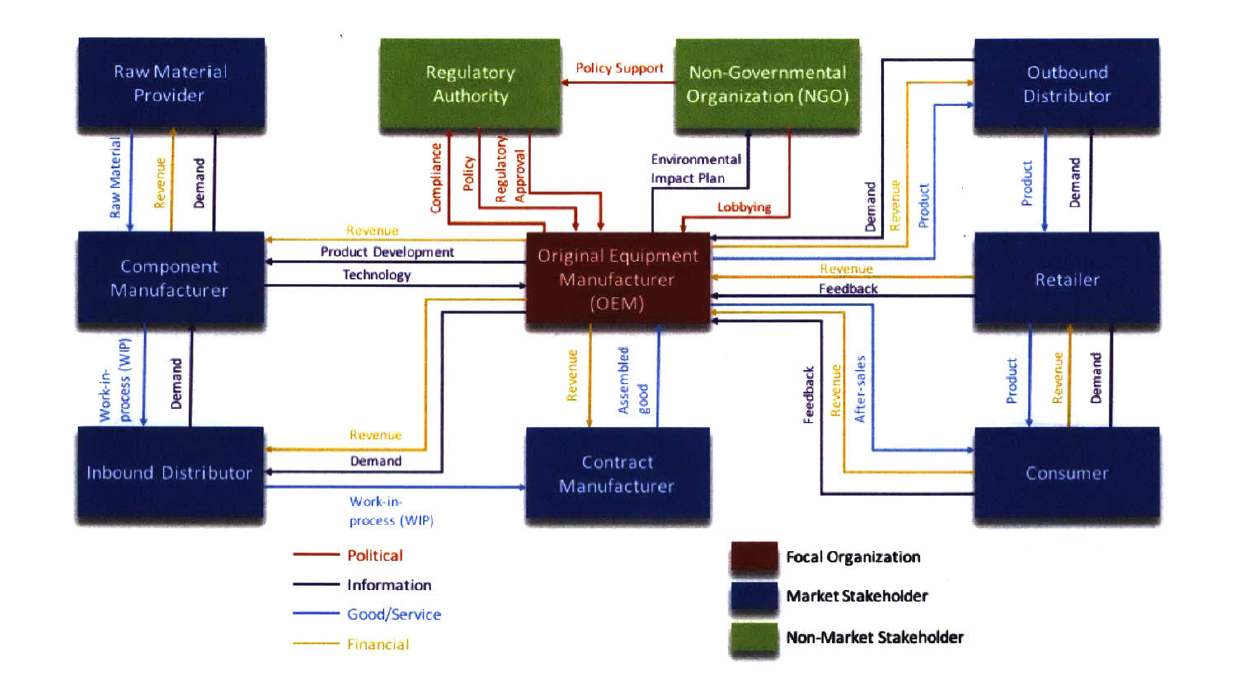
\includegraphics[width=1.45\textwidth]{images/chap03_stackholders.png}
		\end{minipage}
		\caption{Stack holders network for a generic supply chain}
		
	\end{figure}
	
\end{center}

\begin{itemize}
	\item \textbf{OEM: } Original Equipment Manufacture has key role among all stack holders. OEM has multiple tasks such as forecasting demands of customers, inventory management, control flow and product development and marketing. In fact, the main goal of OEM is to develop product, distribute them, observe satisfaction of customer by fulfilling their demands.\\
	\item Raw-material: it is the first phase in supply chain where it's responsible for providing the raw material for manufacture providing high quality of raw material.
	\item Component Manufacture: raw material is used by component manufacture to produce component with high quality and earn revenue and trust of OEM in return.
	\item Inbound Distributor: Obtain component from manufacture to distribute it to contract manufacture assembly.
	\item Contract Manufacture: the OEM can choose to outsource final assembly to a contract manufacture to build product.\\ 
	\item Outband Distributor: it receives final product from OEM and distribute it to retailers for sale.
	\item Retailer: It is responsible to sale the product to customer. Maximize sale of product and enhance the quality of products.
	\item Customer: It is the end of supply chain process and is main source of demand.
	\item Authority: Is non market stackholders and has main role in this process to ensure that products meet requirements and minimize danger.
	\item Non-Governmental Organization(NGO): It is a non-market stackholder that have impact on product. Their goal is to public awarness of issue and increase their popularity\cite{Angwei}.  
	
\end{itemize}
\section{Challenges encountered in Supply chain}
As supply chain is long and complex process. There are some challenges which segregated into two types:\\
\begin{itemize}

\item \textbf{Planning stage:}\\
It deals with forecasting the customer demands from one hand and inventory management on the other hand. 
\textit{Demand prediction} is the main challenges in supply chain. Supply chain develops some models to deal with this issue. As the demand of customers change overtime.
Supply chain build up some models and analysis methods 
to predict demand using data and other characteristic.  \\
\textit{Inventory management}, supply chain tries to keep balancing between supplier and customer. If supply chain is too low, client and customer relationship will be affected negatively. If supply is too high, that will have much inventory and it costs lower price. Apart from all, the most important thing in this process is time managing to minimize delay and delivery time to customer. Supply chain build some models to fill the inventory to maximize profit and minimize costs.

\item \textbf{Coordination stage}:
Due to multiple stockholders in supply chain, it exist information inconsistency. Lack of information poses some challenges in supply chain that we referred to some of them. It affected the product traceability negatively.Lack of real time information to track the product, it is difficult to update demand prediction and consequently destroys the trust between stack holders. One suspects information is being held by others and so on.\\ 
In addition, The product quality and information sharing hold the business structure together,that allow supply chain to improve coordination and product quality, manage the risk or distribution due to natural catastrophe\cite{Angwei}. 
\end{itemize}
\section{How to improve challenges using smart contract?}
Supply chain used smart contract to deal with three concerns:\\
1- Provenance of goods\\
2- Good traceability\\
3- Using open database to build trust between stack holders\\
To determine \textbf{provenance}, Supplier A(main supply chain) records the detail of raw material by the usage of smart sensor the location of materials and time of shipping can be stored into blockchain which will be available to all parties.\\

Using the provenance the source of product will be verification for all parties. In order to \textbf{tracking} the product, all parties should record all detail of shipment in blockchain. Whenever a good received on the specific location, contract will be triggered to shipping party. The task of OEM is to determine time and location of shipping .\\
\begin{center}
	
	\begin{figure}[htb!]
		
		\begin{minipage}{0.55\linewidth}
			\centering
			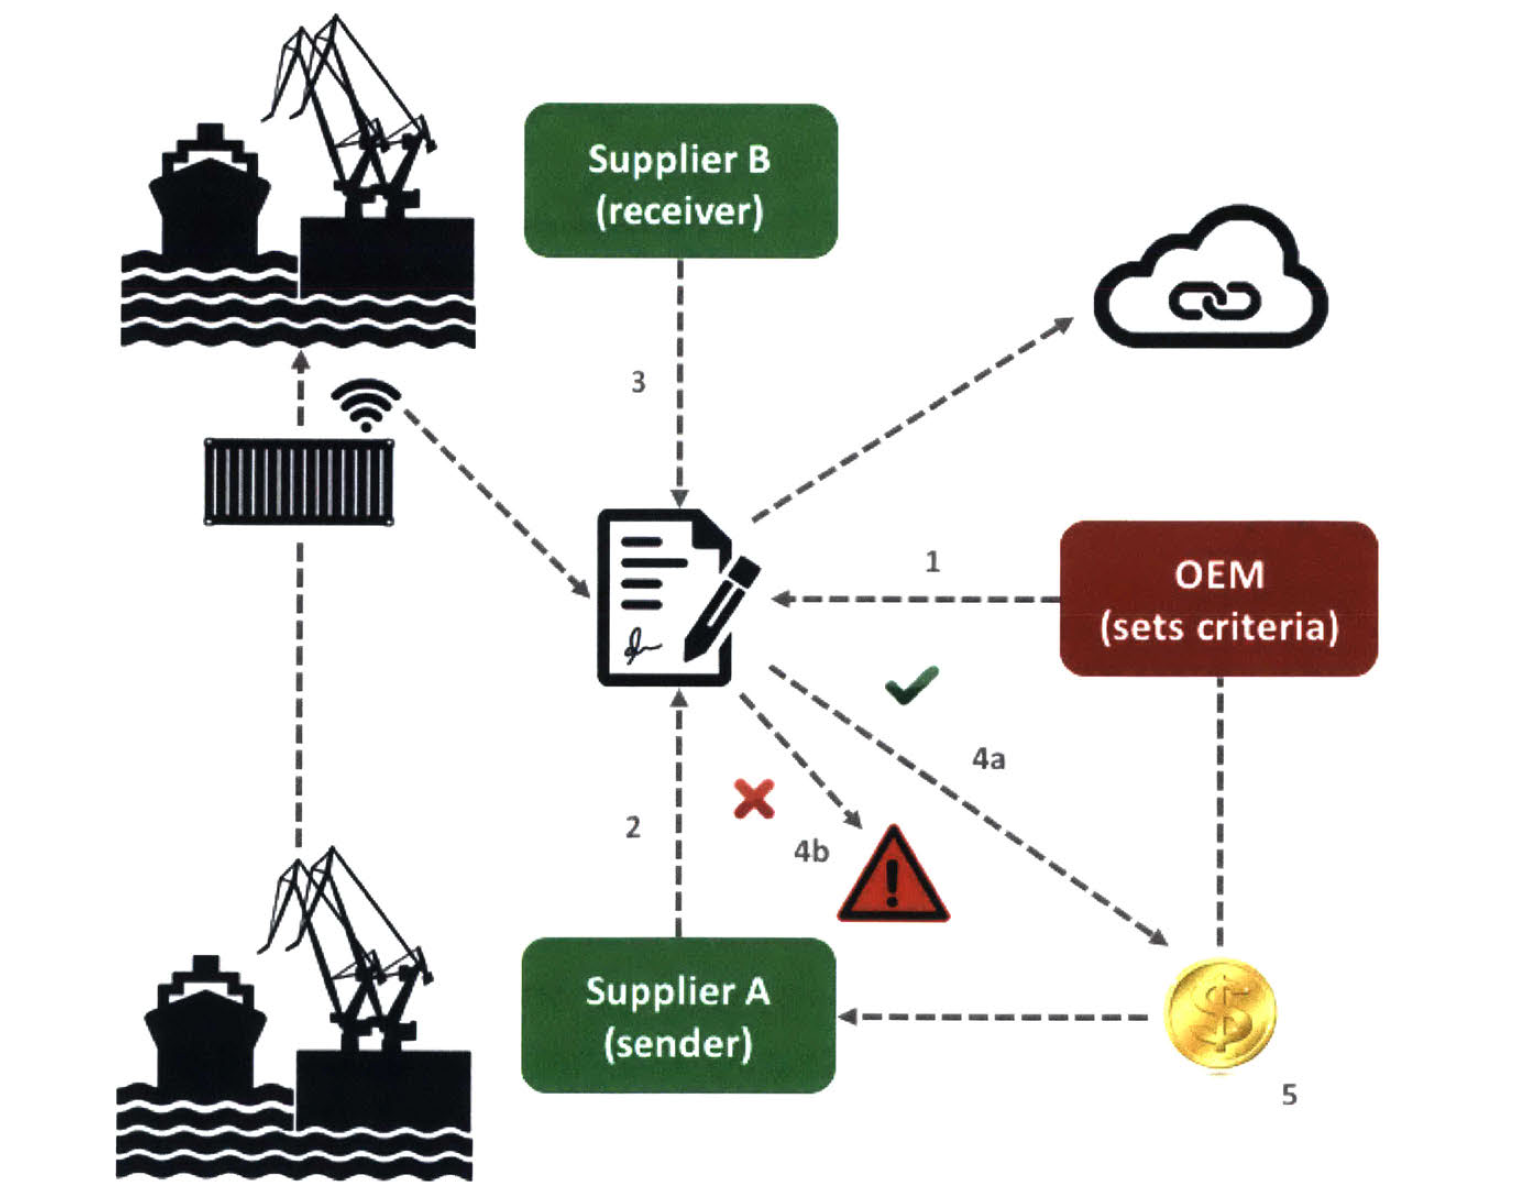
\includegraphics[width=1.65\textwidth]{images/chap03_tracking_SCM.png}
		\end{minipage}
		\caption{Using smart contract to track the goods in supply chain management}
		
	\end{figure}
	
\end{center}

Supplier A, send shipment to Supplier B and record on blockchain. Supplier B also records on blockchain by receiving shipment. Smart contract then check whether all predetermined obligations are met.
Afterward,  payment will carry out otherwise, an alert is triggered to parties to eliminate problems.  Automate tracking helps to simply the supply chain process and update states. That's why the supply chain will be more agile to un-predicted situations.\\ 
As already said, supply chain is\textbf{open database} where all parties can store the detail of information in blockchain. By every shipment, the reputation or credit of parties will increase which would be included smart contract for tracking goods. When smart contract call a contract for an transaction,  score (credit) also be accessible. The open database help smart contract for more transparency\cite{Angwei}.

\subsection{proof of concept development }
Tracking contract let the parties to trace the shipment of goods and execute the payment automatically once shipment is completed and predetermined conditions are met. In smart contract event used to display message when the transaction is executed. Smart contract here consist of some functions as follows:\\
\textbf{getBalance} it allows to parties to check the balance of an account by inserting public address.\\
\textbf{arrived}: is an alert function which show the mount of goods and address, whenever good arrive to destination.
\textbf{arriveGood} it allows receiver records all detail of goods on blockchain once goods are received. Receiver check whether the items are receive are match with those are shipped. if they match, an event is triggered that the item has been received successfully otherwise it fails.\\
\textbf{sendGood} sender records all information about goods as soon as goods departure. A mapping is used to map the tracking the goods like address quantity and item. Also goods is traced with real time location using sensor and other information such as time and address recorded into blockchain. An event will be triggered as item has been shipped.\\
\textbf{checkSuccess} This allows to any of parties to check the number of successfully shipment.
\textbf{getDetails}: Gets all the details for the package contract in a call and returns all of the public members of the contract. 

\subsection{Smart contract Validation}
Remix IDE is browser-based compiler that enables users  to compile contract  with solidity code. It simulates EVM  to execute smart contract and debug it.  As executing smart contract on Ethereum costs some
ether, Remix provides an environment to compile and debug it without any transaction fee. \textit{Figure 3.5} Figure 3.5 represents a screenshot of the Remix IDE, where  cost of executing a
contract (goodTracking.sol), transaction (sendGood)and it's output are represented: 
  

\begin{center}
	
	\begin{figure}[htb!]
		
		\begin{minipage}{0.55\linewidth}
			\centering
			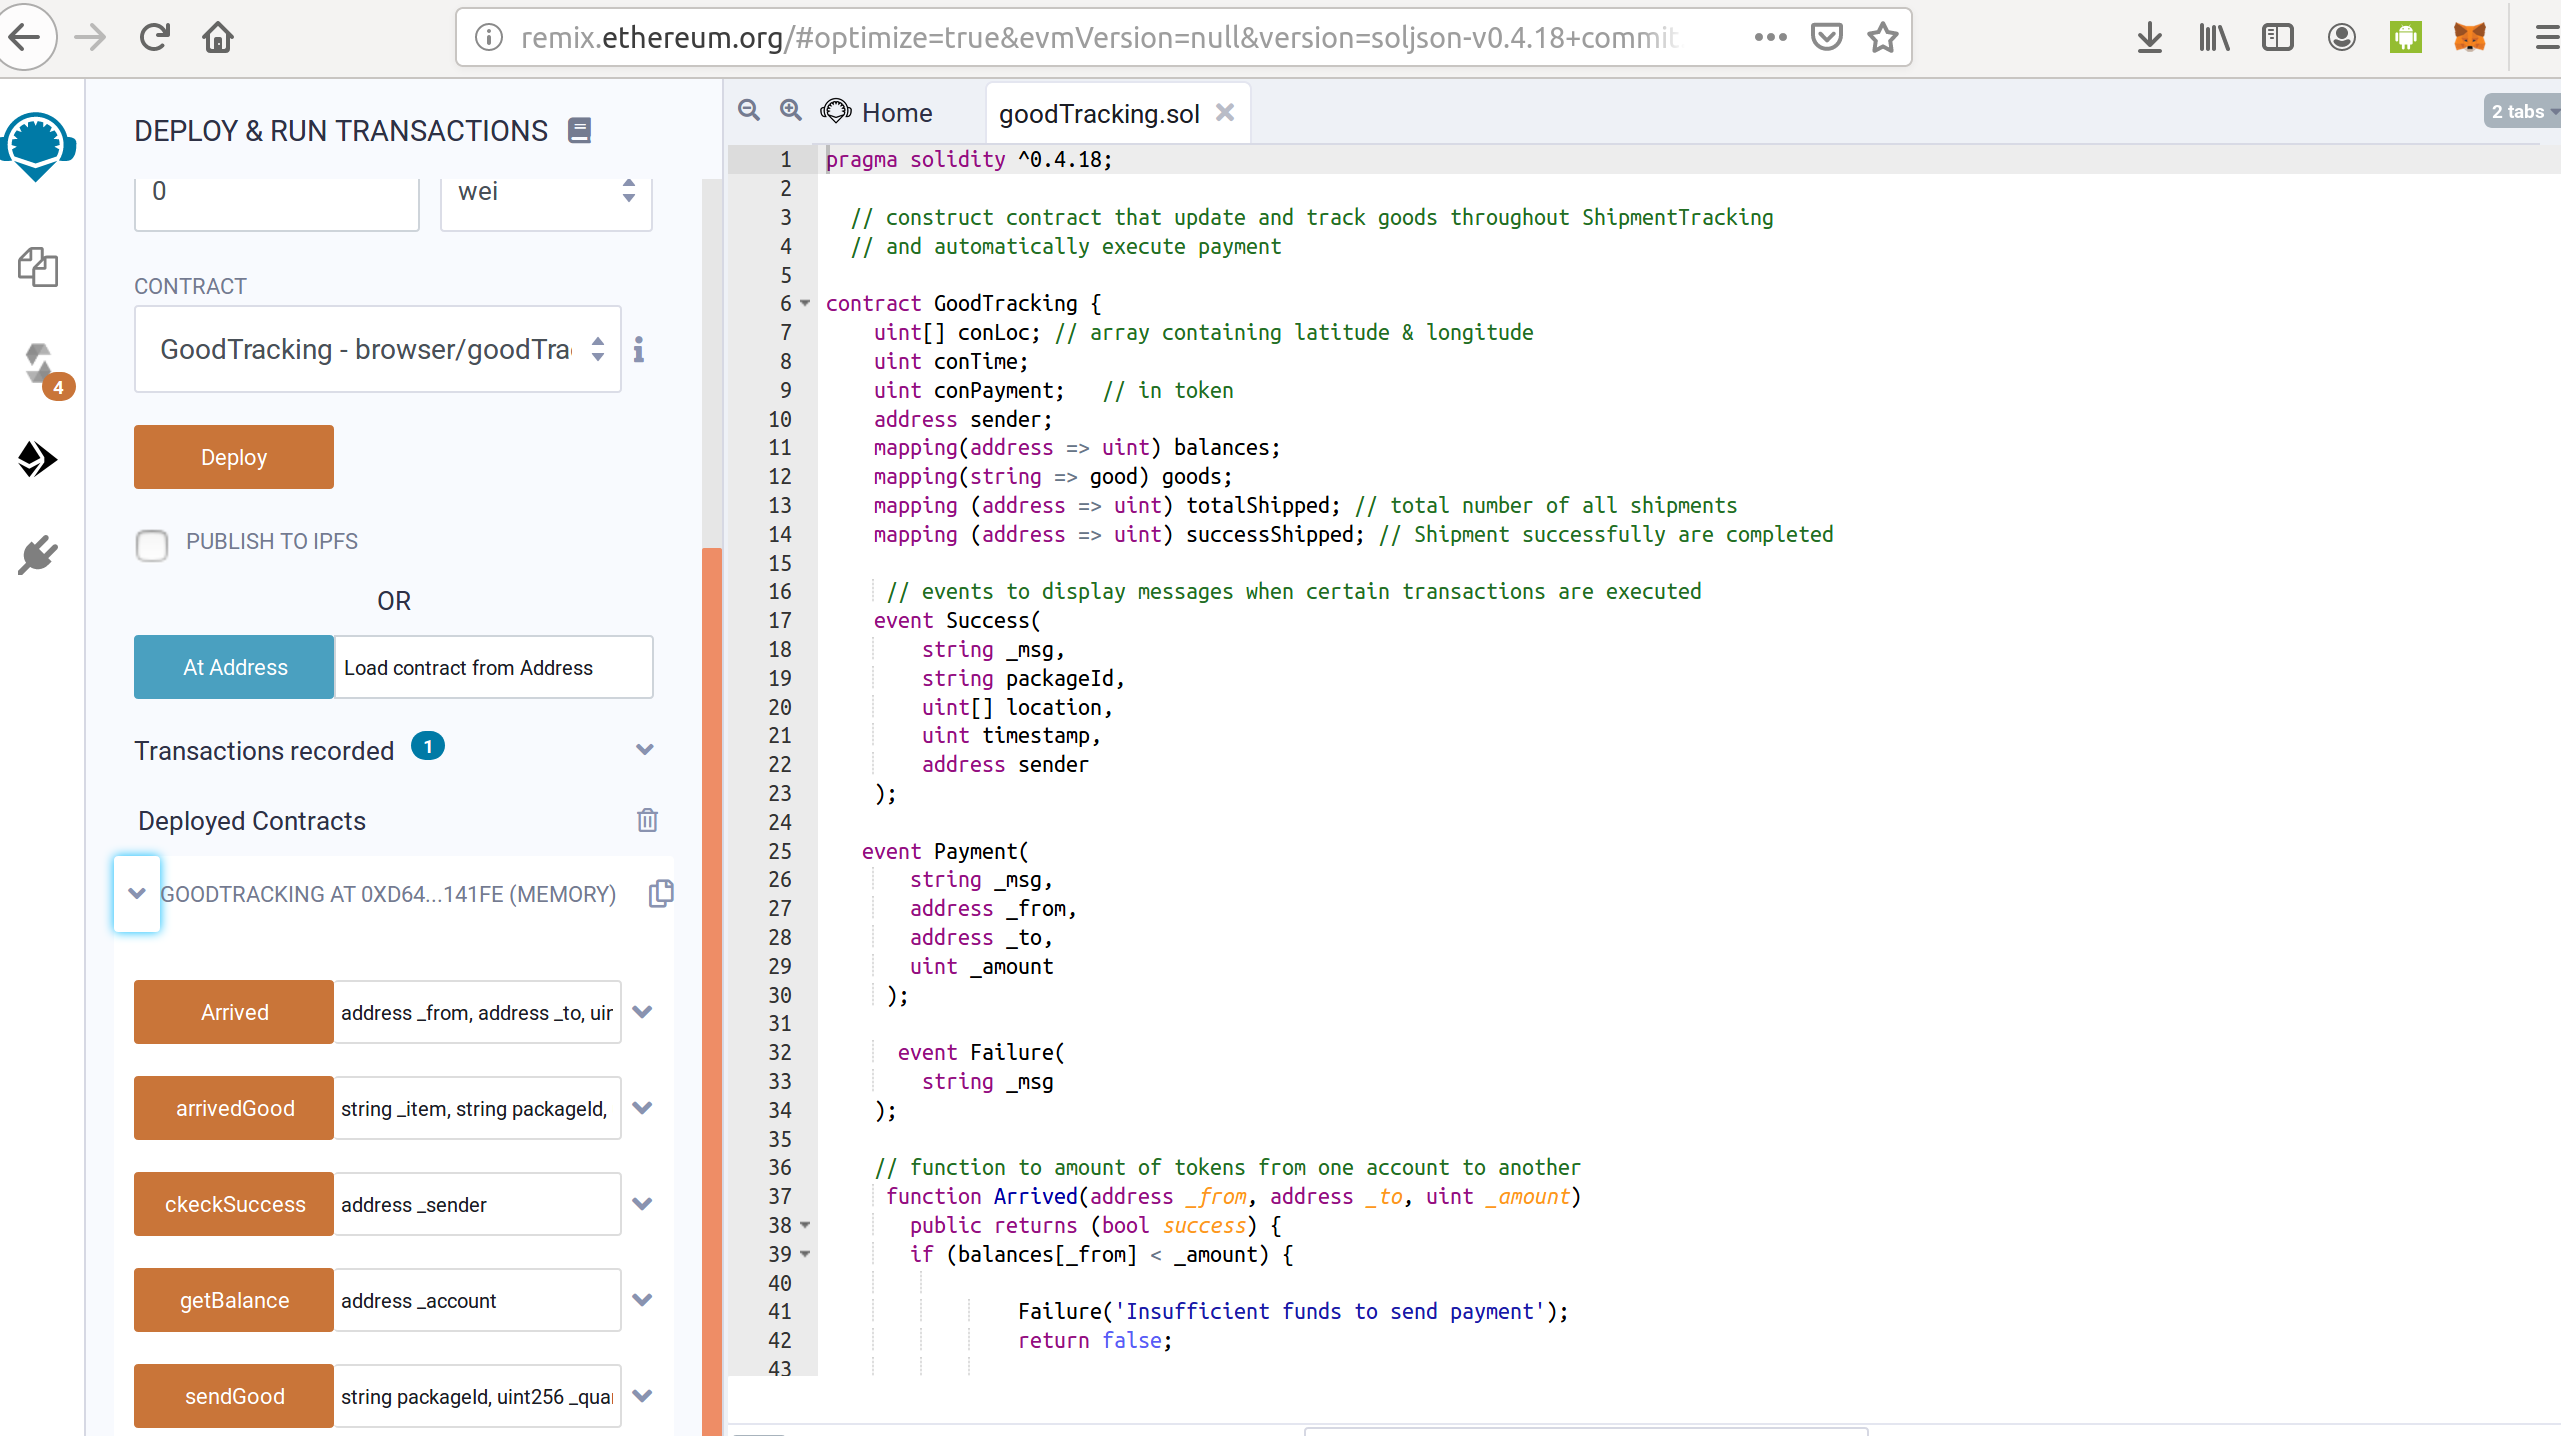
\includegraphics[width=1.55\textwidth]{images/chap03_remix.png}
		\end{minipage}
		\caption{Remix IDE to deploy shipment tracking smart contract}
		
	\end{figure}
	
\end{center}

To validate smart contract, the contract deployed with some tokens to administrator. Admin sets contract to ship good from supplier $A$ to supplier $B$. When supplier $A$ send good and record detail on blockchain. When supplier $B$ receives good, records detail also on blockchain. When the shipping quantity is not matched, an alert is triggered and fail smart contract to deploy.

\begin{center}
	
	\begin{figure}[htb!]
		
		\begin{minipage}{0.55\linewidth}
			\centering
			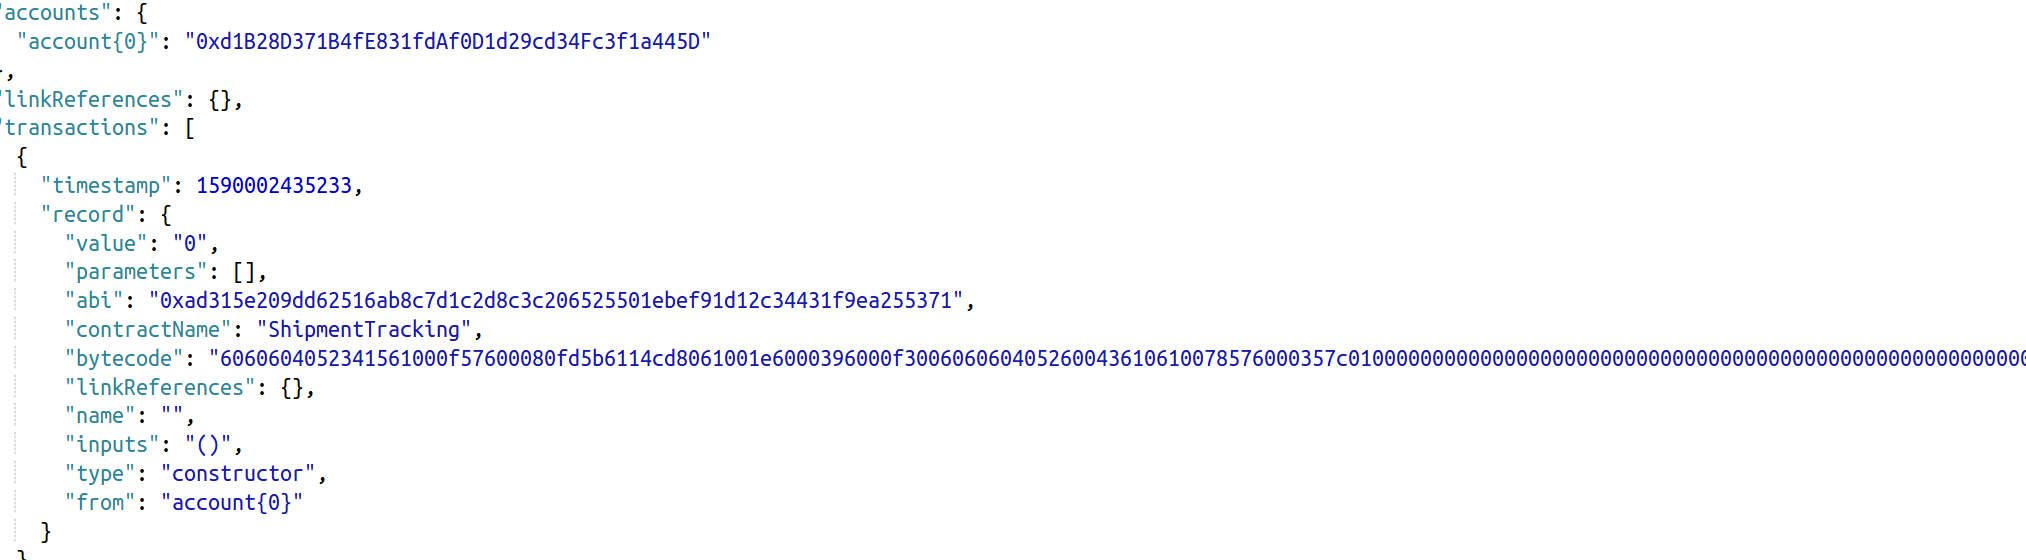
\includegraphics[width=1.55\textwidth]{images/chap03_ABI.png}
		\end{minipage}
		\caption{Recorded transactions after deploying smart contract}
		
	\end{figure}
	
\end{center}


\section{Semantic Blockchain development Implementation}
There are limited work integrating semantic in blockchian specially smart contract.There exist only some work on Ethereum ontology which describe blockchain concepts using RDF schema and OWL. In this analysis used Ethereum ontology which describes basic semantic concepts related to specific schema such transaction or blocks. I used specific concepts to transaction that i used in this study.\\
EthOn represent different models such as block, account, smart contract concepts, instances and relation.
Ethereum ontology covers concepts and relations between objects. As my goal is to extend ontology to support my favorite schema based on dataset by mapping to EthOn blocks or transactions model.\\
EthOn describe concepts, block, transaction in machine readable format that can facilitate reasoning which can be supported our semantic web service description
Some possible ways to semantify blockchain:\\
\textbf{Step 1.} Create schema of blockchain or transaction , mapping of these data to RDF make using of vocabularies and remote procedure calls.\\
\textbf{Step 2.} Using blockchain data storage as input that will be mapped based on these data.\\
\textbf{Step 3.} Create properties of all blocks or transactions..\\
\textbf{Step 4.} Mapping all block properties to block dataset and generates output of all inputs.\\
\textbf{Step 5.} Copy output in turtle file where related prefixes are defined.\\
\textbf{Step 6.} Generate output based on SPARQL query and  data produced on previous step.\\

\subsection{Proof of concept}
\textit{Dataset}: The main part of our analysis is the dataset which can be exported by some block explorer such etherscan that is used in this research. Dataset will feed into our Ethereum ontology mapping which each attributes map to responding values of dataset.\\
\textit{Etherscan} is block explorer which allows us to search Ethereum blockchain for transaction, contract, blocks, addresses, price and other activities takes place on Ethereum.\\
\textit{Template} is in the form of RDF triple based on subject predict object that contains prefix of concepts, Ethereum ontology concepts, our schema with the type of concepts in ethOn and instances such as integer, hex binary, boolean and string.\\

\begin{lstlisting}
ibb:{{tx_block_number}} ethon:containsTx tx:{{tx_hash}} .
tx:{{tx_hash}}  ethon:number 
"{{tx_block_number}}"^^xsd:hexBinary .
tx:{{tx_hash}} ethon:blockCreationTime "{{tx_block_timestamp}}"^^xsd:dateTime .	
tx:{{tx_hash}}  ethon:from "{{tx_from}}
"^^xsd:hexBinary .	
tx:{{tx_hash}}  ethon:to "{{tx_to}}
"^^xsd:hexBinary .	
tx:{{tx_hash}}  ethon:address "{{tx_address}}"^^xsd:hexBinary  .	
tx:{{tx_hash}}  ethon:txGasPrice  "{{tx_gas_price}}"^^xsd:integer .	
tx:{{tx_hash}}  ethon:txGasUsed  "{{tx_gas_used}}"^^xsd:integer .	
tx:{{tx_hash}}  ethon:ValueTx  "{{tx_value}}"^^xsd:integer .
\end{lstlisting}

\textit{Mapping function} is used to tripleize and map all the properties of dataset, our schema and Ethereum ontology concept to each other.\\

\begin{lstlisting}
function tripleize (data, template){
let properties = {
tx_hash: (data[0][0]),
tx_block_number: data[0][1],
tx_block_header: data[0][2],
tx_block_timestamp: data[0][3],
tx_from: data[0][4],
tx_to: data[0][5],
tx_address: data[0][6],
tx_gas_used: data[0][8],
tx_value: data[0][9],
	};
\end{lstlisting}

\textit{Tripleize Application} used to feed relative dataset to Ethereum ontology concepts and our schema and integrated data.(See appendix for more detail)
\textit{Header} of output formed the prefix of out concepts.
\begin{lstlisting}
@prefix ethon: <http://ethon.consensys.net/> .
@prefix ibb: <http://ethon.consensys.net/Block#> .
@prefix ibu: <http://ethon.consensys.net/Uncle#> .
@prefix ibs: <http://ethon.consensys.net/State#> .
@prefix tx: <http://ethon.consensys.net/Tx#> .
@prefix xsd: <http://www.w3.org/2001/XMLSchema#> .
\end{lstlisting}
\textit{Sparql} query is an RDF query languages that is semantic query language for dataset- enable to present and manipulate data  stored in Resource Description framework.(see appendix for full source code). \\

\begin{lstlisting}
PREFIX : <http://ethon.consensys.net/>
PREFIX dc: <http://purl.org/dc/elements/1.1/>
PREFIX ns: <http://www.w3.org/2003/06/sw-vocab-status/ns#>
PREFIX v0: <http://ethon.consensys.net/v0/>
PREFIX owl: <http://www.w3.org/2002/07/owl#>
PREFIX rdf: <http://www.w3.org/1999/02/22-rdf-syntax-ns#>
PREFIX xml: <http://www.w3.org/XML/1998/namespace>
PREFIX xsd: <http://www.w3.org/2001/XMLSchema#>
PREFIX rdfs: <http://www.w3.org/2000/01/rdf-schema#>

SELECT   ?class ?p ?o
WHERE
{
?class ?p  ?o

}

\end{lstlisting}

 \begin{center}
 	
 	\begin{figure}[htb!]
 		
 		\begin{minipage}{0.55\linewidth}
 			\centering
 			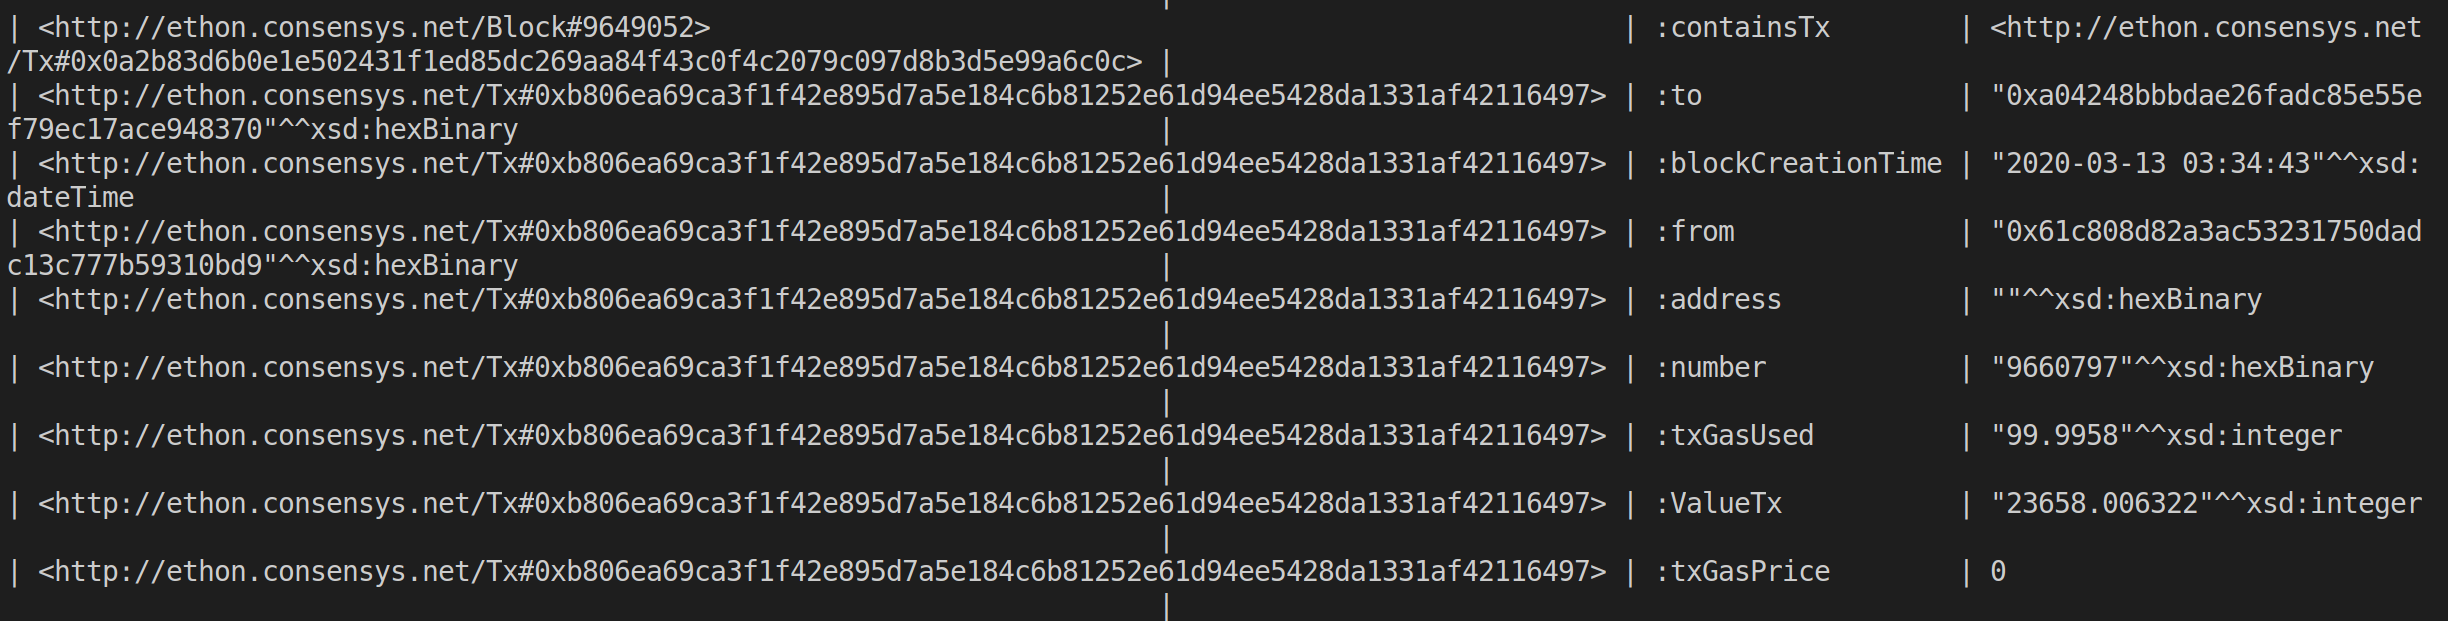
\includegraphics[width=1.55\textwidth]{images/chap03_output_final.png}
 		\end{minipage}
 		\caption{Final output of a transaction based on SPQRL query}
 		
 	\end{figure}
 	
 \end{center}
 